%%% $Id$
%%% Copyright (C) 2002 Greg J. Badros <greg.badros@infospace.com>
%%
%
% This file should be compiled with V1.0 of "www2003-submission.cls"
%
% ----------------------------------------------------------------------------------------------------------------
% This .tex file (and associated .cls V1.0) produces:
%       1) NO Permission Statement
%       2) WWW'03-specific conference (location) information
%       3) The Copyright Line with ACM data
%       4) NO page numbers
%
% ---------------------------------------------------------------------------------------------------------------
% This .tex source is an example which *does* use
% the .bib file (from which the .bbl file % is produced).
% REMEMBER HOWEVER: After having produced the .bbl file,
% and prior to final submission, you *NEED* to 'insert'
% your .bbl file into your source .tex file so as to provide
% ONE 'self-contained' source file.
%

\documentclass{www2003-submission}
\usepackage{times}
\usepackage{moreverb}
\usepackage{floatflt}
\usepackage{url}

\newcommand{\B}{\discretionary{}{}{}}
\newcommand{\smtt}{\small}
\newcommand{\smtexttt}[1]{{\small\texttt{#1}}}
\newcommand{\ns}[1]{{\small\texttt{#1:*}}}
\newcommand{\figref}[1]{Fig.~\ref{fig-#1}}
\newcommand{\secref}[1]{Section~\ref{sec-#1}}
\newcommand{\ssecref}[1]{Section~\ref{ssec-#1}}
\newcommand{\tableref}[1]{Table~\ref{#1}}
\newcommand{\tm}{{\scriptsize $^{\mbox{tm}}$}}
\newcommand{\gjb}[1]{{\sc gjb:}\textbf{#1}}

\newenvironment{smallverbatim}%
{\renewcommand{\baselinestretch}{1}\small\verbatim}%
{\renewcommand{\baselinestretch}{2}\endverbatim}

\begin{document}
%
\title{The Extensible Templating Language: \\
       An XML-based Restricted Markup-Generating Language}

\numberofauthors{1}

\author{
%
% The command \alignauthor (no curly braces needed) should
% precede each author name, affiliation/snail-mail address and
% e-mail address. Additionally, tag each line of
% affiliation/address with \affaddr, and tag the
%% e-mail address with \email.
\alignauthor Greg J. Badros\\
       \affaddr{InfoSpace, Inc., 601 108th Ave. NE, Suite 1200, Bellevue, WA 98004, USA}\\
       \email{greg.badros@infospace.com}
}
\date{12 November 2002}
\maketitle
\begin{abstract}
Popular web templating languages typically embed general-purpose
programming languages.  The Extensible Templating Language was born
out of questioning the fundamental assumption that front-end
markup-generating engine of a multi-tier web application requires all
of the power and expressiveness implied by that design.  ETL restricts
the set of language features to a useful subset that provide the
necessary functionality without compromising the simplicity and
understandability of templates.  Furthermore, ETL improves the
analyzability of the source templates by using an XML-based
representation where markup is intermingled with XML elements
corresponding to programming constructs. This approach reduces the
possibility of generating improper markup, improves the separation
between presentation and business logic, and facilitates tool-building
including semantically-aware editors and debuggers. ETL runs inside of
the Extensible Templating Language Server which is currently employed
by InfoSpace to serve over forty million requests per day using over
sixty thousand ETL templates.

\end{abstract}

% A category with only the three required fields
%% GREGB:FIXME::
%% See http://www.acm.org/class/1998/overview.html
\category{D.2}{Software}{Software Engineering}
\category{D.3}{Software}{Programming Languages}

% GREGB:FIXME:: any terms?
%\terms{}

\keywords{Restricted domain-specific programming language, static analysis,
web server, templates, XML, XSLT, markup, WML, HTML.}

\section{Introduction}
\label{sec-intro}

The loosely-coupled client/\B{}server model implied by the current
breed of applications deployed via the World Wide Web presents
substantial new complexities for application developers. A variety of
new programming languages and paradigms attempt to address these novel
problems.  One important characteristic of this new world of software
development is the need to generate HTML, WML, or other markup
languages to describe client-side presentation and behaviour.

The original server-side dynamic markup-generation capabilities of the
Web were defined by the Common Gateway Interface.~\cite{CGI11} For each
request of a CGI, the web server maps HTTP request details into environment
variables, command-line arguments, and the standard file descriptors.
In particular, the standard output written by that process was sent by
the Web server as the response to the client browser (instead of
simply responding with an unchanging file from disk).  Over time,
various techniques arose to reduce the cost of each request: extension
mechanisms such as the Apache module system~\cite{Apache} and
scripting languages hosted by the Web server have increased
performance by eliminating process creation overhead.

Today, server-side markup generation is dominated by expressive and
flexible general-purpose programming languages such as
Java~\cite{Arnold98}, Perl~\cite{Camel3rd}, and PHP~\cite{pro_php}.
Ironically, the languages are then mostly used
in fairly restricted ways, often being tied to a templating syntax
(e.g., JSP~\cite{JSP12} for Java or
HTML::Template~\cite{HTML-Template} or Mason~\cite{Perl-Mason} for
Perl).  For example, consider the PHP template in \figref{php-books}.
The only constructs required by the template are a) some means of
populating a data model from the back-end business logic (line 1); b)
data-driven iteration (line 4-5); and c) simple expression evaluation
to access parts of the data model (lines 7 and 9). The extra power
provided by typical templating languages not only goes unused, but it
also complicates certain important analyses of the code.  For example,
the obviously important property that a template execution terminates
is undecidable for these general purpose languages.  

% GREGB:FIXME:: check the above line numbers 

\begin{figure}[tb]
\begin{listing}{1}
<? $books = GetBooks(...); ?>
<html>
 <table>
  <? for ($i = 0; 
           $i < count($books); ++$i) { ?>
   <tr>
     <td><? print($books[$i][author]); ?>
         </td>
     <td><? print($books[$i][title]); ?>
         </td>
   </tr>
  <? } ?>
 </table>
</htm>
\end{listing}%$
\caption{Cleanly-written PHP templates require only the simplest
programming language constructs.  Unfortunately, over the evolution of
the presentation layer, PHP developers sometimes engage in far broader
interactions because the power of the language allows them to do so.
\label{fig-php-books}}
\end{figure}

For most contemporary web application development frameworks, the
restrictions desired of the front-end templating layer are imposed
only by process and convention.  Template authors are asked to limit
themselves to a subset of the available features of a language as a
means of facilitating scalable, secure, well-behaved systems.
Importantly, however, there is nothing inherent that prevents
template-based code from, for example, making individual database
connections (which would impact performance) or maintaining
undesirable server-side state (which would impose additional
requirements on the load-balancing mechanism and reduce scalability).
Languages such as PHP encourage the undesirable mixing of front-end
presentation with back-end business logic.~\cite{Crane2002} That
approach is counter to the goal of many development organizations to
force a strong separation between the web developers and back-end
application developers. While web developers have substantial
expertise in HTML, user-interface design, and client-side scripting,
their responsibilities often do not include consideration of the
larger architecture.

Another substantial problem with existing templating technologies is
that they often involve the lexical mixing of two separate programming
paradigms.  JSP, for example, is implemented in terms of a
pre-processing rewrite of the template into a Java servlet.~\cite{JavaServlet23}
Pre-processing approaches are convenient for programmer expressiveness
but have a huge hidden cost in complicating software engineering
analyses and tools that would otherwise help understand, maintain, and
evolve the complex systems~\cite{Badros00-spe,ErnstBadrosNotkin02}\cite[p.~424]{Stroustrup94}.
The precise analysis of an arbitrary JSP template necessarily requires
full knowledge of both the rewrite rules and the semantics of Java.

\subsection{Restricting the language}

All popular markup templating languages integrate with a
general-purpose programming language.  This approach offers numerous
advantages.  For example, undoubtedly the language is sufficiently
powerful and expressive for the needs of markup generation.
Additionally, numerous language-level tools such as compilers and
debuggers, are already available for the templating language to
leverage.  Certainly for platform providers that have a large
investment already made in a general purpose language, it is natural
to extend that investment to a templating language.\footnote{XSLT can
be used in a templating style~\cite[2.3]{XSLT}, but popular use of
XSLT also leverages scripting extensions to deal with the far too
severe restrictions of the language.}

Despite the broad assumption that a markup language requires the use
of a general purpose programming language, an obvious alternative
exists: use a domain-specific language specifically tailored to the
needs of generating markup.  Such an approach can mitigate several of
the problems mentioned previously.  In particular, using a restricted
programming language at the front-end to generate markup can enforce
better separation of front-end presentation from back-end application
logic and may simplify the templates such that they are easier to
write, read, and evolve.

\begin{figure}[bt]
\begin{centering}
\includegraphics[width=1\linewidth]{web-service-ip-shift.eps}
\caption{Web services enable the front-end templating tier to
communicate with back-end applications via standard Internet Protocols
such as XML and SOAP; they no longer need to be aware of distributed
object protocols such as DCOM or Corba.\label{fig-ws-ip-shift}}
\end{centering}
\end{figure}

If we limit the functionality of a markup templating language, one
capability that remains important is accessing back-end applications.
The architecture of the classic three-tier application appears at the
top of \figref{ws-ip-shift}.  Historically, the communication between
the front-end and back-end servers uses an object-oriented data model
and involves remote procedure call mechanisms such as DCOM or Corba.
As the web service architecture depicted in the bottom of
\figref{ws-ip-shift} increases in popularity, the need for the front
end templating language to reason about language-level objects is
reduced.  Instead, the XML data model implied by web services can be
the primary communication format and the front end need only use
Internet standards such as HTTP and XML in interacting with other
applications.  This observation simplifies the requirements
for front-end markup templating languages and supports the possibility
that a restricted programming language may suffice.

%% GIVE EXAMPLES OF VALUABLE ANALYSES!!!
\subsection{Analysis of markup templates}

Templating languages have one primary goal: to generate markup to be
returned to the requesting user agent.  It is important that the
markup created conforms to appropriate Internet standards.  For
example, WML markup needs to first be well-formed XML and second be
valid with respect to the appropriate schema or DTD~\cite{WML12}.
Although HTML browsers are more forgiving of variations in syntax,
best-practices still dictate that the markup returned be in compliance
with the HTML specification~\cite{HTML4}.  Popular templating
languages including PHP, JSP, ASP, and others all process arbitrary
text and are ignorant of the rules of the markup being generated: the
mistaken close tag on line 14 of \figref{php-books} goes unnoticed by
PHP.

Tools such as HTMLTidy~\cite{HTMLTidy} are available to check the
responses from servers for conformance, but often testing involves
simply using various browsers to exercise the application while
looking for bugs.  Both of these approaches require exhaustively
visiting every page of interest--often a very large search space.
Ideally, we would prefer a way to statically analyze the source templates
themselves to gain confidence that they will, in fact, generate proper
markup.  If static analysis of templates can rule out the possibility
of certain kinds of errors, testing time and costs can be dramatically
reduced.

Another important requirement for software development systems is to
support ad-hoc queries of the source code. For small and simple
dynamic web applications, the automated analysis of templates is often
unnecessary: a web developer or two understands all of the code.  Over
time, however, these simple applications grow in size and complexity
such that tools analyzing the templates become an essential part of
maintaining and evolving the system. For example, a site may wish to
add an extra input field to all of its registration forms.  If a
generic form is not already factored out into a common location, the
first step in approaching the task is finding all of the registration
forms.  Or suppose a new handheld device has a limitation in its
handling of cookies: we need a means of narrowing the scope of careful
review to places where that cookie is manipulated.

Typically, web developers approach to above scenarios with an arsenal
of imprecise lexical tools such as \smtexttt{grep}.  While searching
for a substring or regular expression may satisfy some simple queries,
when the desired query has additional structure, lexical approaches
fall short.  Suppose we wish to find dead code to simplify our
application. No regular expression will let us identify all
unreachable templates to satisfy that query.  To analyze more deeply,
we need to uncover the semantic structure of the templating language.
Typically, that requires a language-specific parsing approach and much
greater effort in building a valuable tool or an extensible integrated
development environment~\cite{Soroker97,Eclipse}.

\subsection{XML supports analyses and tools}

An increasingly popular approach to performing structured queries of
programming language source code is to use standard XML tools such as
XSLT~\cite{XSLT} and XQuery~\cite{XQuery} to operate over a
complementary XML-based representation~\cite{Badros-www9,Schonger2002,Gondow2002,Power2002}.
With a carefully-chosen XML representation, valuable semantics of the
code are immediately available to XPath expressions, thus facilitating
a broad class of source code tools.  However, for a general-purpose
programming language, XML is unwieldy for use as the primary
representation.  Instead, the conventional grammar-based language is
edited by humans and is only converted into XML for the tools to
leverage.

This research applies the benefits of an XML representation of source
code to the domain of restricted markup templating languages.
Importantly, web developers working with templating languages are
already writing markup directly, thus making it natural for them to
express the limited logic of their dynamic templates directly in
markup as well.  This observation eliminates the dual representation
problem that restricts the value of XML when applied to general
purpose programming language.  The approach also enables the use of
schema-aware XML editors to provide a rich development environment
with very little ETL-specific effort (see \secref{benefits}).

In this paper, I introduce the Extensible Templating Language.  From
one perspective, ETL is a 100\% XML-based templating language that
embeds programming language constructs directly in the XML
representation, intermingled with literal target-language markup.
Alternatively, we can view ETL as an imperative domain-specific
programming language that uses XML as its surface syntax and
simplifies the writing of programs that generate markup languages.

ETL leverages the well-formedness and local-validity checks of the
source template to support those same properties in the generated
response markup.  By limiting the programming-language constructs to
include only the features that are appropriate at the front-end of a
scalable web application architecture, we ease numerous analyses and
encourage proper separation of the presentation from the content and
business logic. Finally, because of its use of XML as a
representation, ETL simplifies ad-hoc software engineering analyses to
better support evolution and maintenance of large dynamic web
applications.  We have built an ETL runtime inside of a
production-quality web server, the Extensible Templating Language
Server.  ETLS is currently employed by InfoSpace to serve over forty
million requests per day using over sixty thousand ETL templates.

\subsection{Outline of paper}

The rest of this paper is organized as follows. \secref{etl} describes
the Extensible Templating Language itself. \secref{benefits} gives
several practical examples of the benefits of using a pure XML
approach with a restricted programming language.
\secref{implementation} details our implementation and
describes our experiences in using ETL in production systems over the
last year.  Finally, \secref{related-work} describes and contrasts
related work and \secref{conclusion} concludes.

%%% 
%\section{Background}
%\label{sec-background}

%% JSP/XML
%% XSLT

%\subsection{Current templating strategies}

%\subsection{Comparison of approaches}

%\begin{table}
%\centering
%\caption{Summary of existing templating approaches.}
%\begin{tabular}{|c|c|l|} \hline
%\\ \hline
%\hline\end{tabular}
%\end{table}


%%% 
%% GREGB:VISUAL:: avoid too obvious of an overfull hbox below
\section{\hspace*{-.1in}Extensible Templating Language}
\label{sec-etl}

The Extensible Templating Language is an imperative markup templating
language that allows web developers to intermingle literal XML markup
with XML-based programming language constructs.  Our primary design
goals for ETL were to:\footnote{A fifth important design goal was to
enable automatic translation of our legacy templating language into ETL. That
need occasionally complicated our design. This bulk of this paper
focuses on the essential language, and
\secref{implementation} mentions our migration to ETL a bit more.}

\begin{enumerate}
\item Allow easy analyses of source templates to permit development of
supporting tools; 
\item support only the essential programming language constructs
required by a templating layer; 
\item focus on an imperative (i.e., procedural) programming model; and
\item utilize an XML data model pervasively to integrate seamlessly
with Internet and Web standards.
\end{enumerate}

An ETL template must be well-formed XML that is valid with respect to
several XML Schema Definitions.  The set of programming constructs
available in ETL is intentionally restricted to limit the amount of
logic performed in the front tier of a multi-tier web-delivered
application and better enforce proper separation of presentation from
content and business logic.  ETL is used by dozens of production
applications serving over forty million requests per day, thus
providing constructive evidence that the set of available constructs
is sufficient for real-world use.

\begin{figure}[tb]
\begin{listing}{1}
<?xml version="1.0"?>
<bl:template xmlns:bl="http://www....">
 <bl:set var="#xml/books">...</bl:set>
 <html>
  <table>
   <bl:for-each var="#xml/books/book">
    <tr> 
     <td><bl:get var="@author"/></td>
     <td><bl:get var="@title"/></td>
    </tr>
   </bl:for-each>
  </table>
 </html>
</bl:template>
\end{listing}%$
\caption{The ETL template corresponding to \figref{php-books}'s PHP
code is required to be well-formed XML.  Thus, the developer
avoids the mistake from line 14 of the PHP example.
\label{fig-etl-books}}
\end{figure}

Because ETL is 100\% XML and because the language is not a full-blown
general purpose programming language, analyzing ETL templates for
various properties or searching for certain constructs is very well
supported.  In particular, because of the way literal markup is mixed
with programming constructs, the well-formedness requirement on the
source template greatly reduces the probability of common mistakes
including mismatching tags.  Additionally, we can also perform local
validity checks on literal markup elements to confirm their proper
nesting and that they use the correct attributes.  A goal of ETL is to
make approximate analyses easy and precise analyses possible.

An example ETL template appears in \figref{etl-books} and is analogous
to the PHP example from \figref{php-books}.  The program is simply an
XML document with root element \smtexttt{bl:template}\footnote{We use
namespace prefixes consistently to unambiguously refer to elements in
the distinguished namespace URIs recognized by the ETL server.}  The
template contains other elements in the \ns{bl} namespace which we
call ETL \emph{primitives} (see \ssecref{primitives}).  Additionally,
the template can contain markup from arbitrary other namespaces which
we call \emph{literal result markup} (see \ssecref{literal-markup}).

ETL templates are processed within the context of an HTTP request.
The path specified in the URL of the request is used to choose a
template from which processing begins (see
\ssecref{template-dispatch}).  URL and POST parameters, cookies, etc.,
are all available to the template (see
\ssecref{buckets}). The primary goal of executing a template is to
generate an HTTP response including the markup document along with the
various HTTP headers such as the content-type, cookie settings, and
other meta-data.  Generally, an ETL template is similar to a method in
a general purpose object-oriented programming language: it can invoke
other templates as subroutines and can also perform subsidiary HTTP
requests to other servers.  In fact, HTTP-bound
web-service~\cite{WebServicesActivity} calls are the primary means of using
back-end application logic.

The remainder of this section informally describes the structure and
semantics of the Extensible Templating Language.


\subsection{Primitives, attributes, and slots}
\label{ssec-primitives}

An ETL primitive is an element in the \ns{bl} namespace that has a
specific well-defined behaviour inside of an ETL template.  Primitives
either output text to the current destination stream (initially the
response document) or perform some side-effect (or both).  For example
the \smtexttt{bl:set} primitive assigns a variable a value without
outputting any text, while the
\smtexttt{bl:http} primitive outputs either \smtexttt{http} or
\smtexttt{https} based on whether the current request arrived over an
ordinary or secure socket connection.

The behaviour of a primitive is parameterized by the various
attributes allowed on that element.  Some primitives, such as
\smtexttt{http} mentioned above, are always empty---they never are
allowed to contain child elements. 
Other primitives are allowed to be non-empty, using the markup generated
by their contained elements as an extra implicit argument.  For example,
in:

\smtexttt{<bl:if var="showcopyright"> (C) 2002 </bl:if>}

\noindent the contents of the \smtexttt{bl:if} are output if and
only if the variable is non-empty.

Many primitives derive their arguments not from individual attributes
but from pairs of attributes that are together called a \emph{slot}.  For
example, the \smtexttt{bl:cr} directive outputs linefeeds, and the
number of linefeeds it generates is determined by a slot called
\smtexttt{count}.  That slot is specified using a pair of attributes:
\smtexttt{count} and \smtexttt{count-var}.  The attributes are
mutually-exclusive: it is a statically-checked error to specify both on
the same \smtexttt{bl:cr} element.  The \smtexttt{count} attribute has
type \smtexttt{xsd:integer} and is used to provide a literal integer
argument to the primitive.  In contrast, the \smtexttt{count-var}
attribute has type \smtexttt{bl:identifierType} (a restriction of
\smtexttt{xsd:string}) and names a variable to evaluate at runtime to
determine the argument to the primitive.  In both cases, the integer
value of the argument is used as the number of linefeeds to generate,
but for \smtexttt{@count} that number is set statically while for
\smtexttt{@count-var} it is determined dynamically (at run-time).

Using a pair of attributes to represent a logical field is a novel
mechanism to improve the type-safety and ease analysis.  The common
alternative is using a small domain-specific language inside the value
of an attribute.  For example, we could have used \smtexttt{count="2"}
or \smtexttt{count="\$num"} to represent the literal number 2 or the
desire to use the current value of the variable ``num'', respectively.
(XSLT's \smtexttt{value-of} element uses this basic approach.)
Unfortunately, when using a single attribute, the type for the
attribute's value must be broadened and is hence less precise.
Additionally, developers must learn various ad-hoc syntactic rules to
ensure full-fidelity of values: how do you express the literal string
``\$num'' when that sequence of characters means a reference to the
variable ``num''?  All analysis tools the become burdened with the
need to handle the case of, say, a backslashed ``\$'' character and
the rest of the quirks of the syntax.

Primitives can, of course, have numerous arguments, some of which are
controlled by slots and others by individual attributes.  When an
argument is allowed to be set only via an attribute instead of a slot,
that parameter of the directive cannot be influenced at
runtime---often this restriction is imposed to permit optimizations or
to improve our ability to support static analyses.  For example,
\smtexttt{bl:get} writes out the value of a variable and has a
\smtexttt{@transform} attribute that supports various encodings or
decodings of the value (e.g., \smtexttt{url-encode} or
\smtexttt{xml-decode}---see \ssecref{transformations}).  We disallow the
use of \smtexttt{@transform-var} because we want to always know from
static inspection what transformations may occur, thus facilitating
some analyses and optimizations.

\subsection{Variables and values}
\label{ssec-variables}

As with all imperative programming languages, ETL has the notion of
variables that can be assigned to and can later have that value
recovered. Variables can be declared inside a single 
\smtexttt{bl:header} element (which is required to be the first element
in a template) and are assigned values using the
\smtexttt{bl:set} primitive. Undeclared variables have dynamic scope and
are live until the end of processing the current request, while
declared variables have static scope and may only be reference in
the same template.  The target variable is named via the
\smtexttt{@var} attribute and the value is given by
\smtexttt{@value}, \smtexttt{@value-var}, or by executing the
children of the \smtexttt{bl:set} element.  For example:

\begin{smallverbatim}
<bl:set var="baseuri"><bl:http/>://<bl:get
 var="hostname"/>/</bl:set>
\end{smallverbatim}

\noindent will set the variable named ``baseuri'' to the value
``http://www.\B{}infospace.\B{}com'' when the request comes as an
ordinary insecure HTTP request and the variable ``hostname'' contains
the value ``www.\B{}infospace.\B{}com''.  While executing its contained
elements, \smtexttt{bl:set} redirects the default output stream to be
used to construct a value to assign to the variable; the output stream
is restored after the child elements are processed (e.g., allowing
nesting of \smtexttt{bl:set} primitives).\footnote{Several other
primitives follow this same pattern.  For example
\smtexttt{bl:set-mime-type} evaluates its contained elements to
generate a value to be used for the MIME content-type of the
response.}  Values are later retrieved by referencing them by name
in a slot, and they can be copied directly to the output stream using
\smtexttt{bl:get}.

ETL has the notion of special reserved variables that may have
side-effects and are used internally for conveying request parameters or
other system-level details.  These reserved variables always start with
the octothorpe (``\smtexttt{\#}'') character and may be read-only (e.g.,
\smtexttt{\#browsertype}) or may alter the behaviour of primitives based
on the value they are assigned (e.g., \smtexttt{\#currencysign}).  
Unlike ordinary variables, there is no guarantee that the value
retrieved from a variable is identical to the value last stored in that
variable.

Various other data is accessible to ETL templates via 
\emph{buckets}. Buckets can be thought of as top-level elements in a virtual
(lazily-evaluated) XML data model that is implicitly available to ETL
templates.  They replace field references and accessor methods of
distinguished objects in languages such as Java.  For example, where a
JSP developer might write:

\begin{smallverbatim}
<%= request.getHeader("User-Agent") %>
\end{smallverbatim}

\noindent the ETL developer accesses the \smtexttt{\#http}
bucket instead:

\begin{smallverbatim}
<bl:get var="#http/User-Agent"/>
\end{smallverbatim}

\noindent Numerous buckets exist in the XML data model providing ways
to access URL parameters, HTTP headers, user settings,
configuration data for applications and brands, and cookies.  Where
appropriate, the buckets are mutable as well (e.g., saving user
settings to the user database).

One additional bucket, \smtexttt{\#xml} is unique in that the values
its variables are bound to are XML DOM trees, not just strings.
When the variable is evaluated in a context that requires a string,
the DOM is serialized to a string as a node is serialized by XSLT when
using
\smtexttt{xsl:value-of}.  Additionally, a trailing XPath expression is
allowed after the variable name when referencing the \smtexttt{\#xml}
bucket.  That XPath expression, when applied to the root element of the
DOM tree referenced by the variable named, must evaluate to a node-set
and the nodes in the resulting node set are serialized in turn to
generate the resulting single string.


\subsection{Transformers \& formatters}
\label{ssec-transformers}

HTTP and XML standards have various different encoding formats to
support arbitrary data over channels that allow limited
representations.  For example, when passing a GET parameter to an HTTP
request, the value is inserted into the URL using an URL-encoding
format that involves (among other things) converting each
\smtexttt{SPACE} character to a \smtexttt{+} character.  To support
such encoding formats in a general way, ETL has defined a set of
``transformers.''

A \emph{transformer} is a streaming converter from one byte sequence to
another byte sequence.  For example, the \smtexttt{url-encode}
transformer converts ``hello world'' into ``hello+world''.  Many
transformers have an inverse that is also supported: the
\smtexttt{url-decode} transformer converts ``hello+world'' into ``hello
world''.  Transformers can be used by ETL code whenever a variable is
being set (via \smtexttt{bl:set}) or accessed (via \smtexttt{bl:get})
using the \smtexttt{transform} attribute of those directives.
Transformers can also be chained together by including the names of
multiple transformers in a whitespace-separated list.  For example:

\begin{smallverbatim}
<bl:get var="a" transform="trim urlencode"/>
\end{smallverbatim}

\noindent results in writing out the value of the variable \smtexttt{a}
after first eliminating leading and trailing whitespace and then
subsequently URL-encoding the resulting trimmed string.  Importantly,
transformation ordering \textbf{is} significant: changing the order to:

\begin{smallverbatim}
<bl:get var="a" transform="urlencode trim"/>
\end{smallverbatim}

\noindent results in a different output string.  If \smtexttt{a} contains
``\smtexttt{ Hello World }'', the former example produces ``\smtexttt{Hello+World}'' while
the latter variant generates ``\smtexttt{+Hello+World+}'' because the
trimming occurs on the URL-encoded string which already has spaces
replaced by plus (``\smtexttt{+}'') characters.

\emph{Formatters} are similar to transformers, but their input is a streaming
virtual XML document (similar to SAX, the Simple API for XML~\cite{SAX})
and their output is a text stream.  Numerous primitives that generate
XML as their output have a \smtexttt{formatter} slot that names the
formatter to use. Several built-in formatters exist, but the most
important feature of formatters is that they can name an XSLT
transformation file.   The events will be used to directly construct a
DOM tree that is then transformed via the named stylesheet, letting the
stylesheet generate the formatter's response string.

\subsection{Control flow}
\label{ssec-control}

There are four primary means of control flow in ETL: template
selection, conditionals, exceptions, and remote invocations.  

\subsubsection{Template selection}
\label{ssec-selection}

Requests made of the ETL server always have an associated abstract
``brand''.  The brand can be explicitly specified as part of the URI
itself, or can be implicit based on the \smtexttt{Hostname} header of
the HTTP request (e.g., when multiple hostnames or domains refer to
the same server).  That brand identifies the customer for whom ETLS is
generating the page.\footnote{This branding feature is heavily
influenced by InfoSpace's business model of building a site once and
customizing it often for different partners.}  The brand is used to
select which template is invoked for the initial processing of a
request and whenever the \smtexttt{bl:call} primitive is used to
execute another template as a subroutine.  

For example, an \smtexttt{index.htm} page may \smtexttt{bl:call} a
\smtexttt{header.htm} template to output a banner for the top of a
page, then do some work to generate the meat of the page, and finally
invoked \smtexttt{footer.htm} to generate another banner for the
bottom.  The \smtexttt{header.htm} at the top-level of the brand
hierarchy may provide some basic functionality, while a sub-brand may
provide an overriding \smtexttt{header.htm} implementation that
specializes the banner for that customer.  The hierarchical
relationships are mirrored in the directory structure of the webtree,
and template selection is analagous to method dispatch in
object-oriented programming languages.  Importantly, ETL only permits
bounded recursion, thus avoiding the possibility of infinite
recursion.

\subsubsection{Conditionals}

Both \smtexttt{bl:if} and
\smtexttt{bl:choose}/\smtexttt{bl:when}/\smtexttt{bl:otherwise}
constructs are supported by ETL and behave much as they do in XSLT.
The primary difference is that ETL does not permit the generality of a
domain specific expression language, and instead uses pairs of
slots to represent the guard conditions.  For example:

\begin{smallverbatim}
<bl:if var="pagenum" less-than-var="max-page">
   <a href="...">Next</a>
</bl:if>
\end{smallverbatim}

\noindent Although this is more verbose than a domain-specific
language in a \smtexttt{test} attribute, it does make it easier to use
XPath to find occurrences of specific operations being used in
conditional guards.   Additionally, it allows us to specify the
left-hand-side value of a comparison guard in \smtexttt{bl:choose} to
specialize that construct into something similar to a
\smtexttt{switch} statement:

\begin{smallverbatim}
<bl:choose var="pagenum">
  <bl:when less-than="1">...</bl:when>
  <bl:when equals="1">...</bl:when>
  <bl:when greater-than-var="max-page">...</bl:when>
  <bl:otherwise>...</bl:otherwise>
</bl:choose>
\end{smallverbatim}

\noindent where each of the \smtexttt{bl:when} clauses compares the
same variable (without needing to redundantly specify its name) .

\subsubsection{Exception handling}

Some primitives throw run-time exceptions.  For example, assigning an
ill-formed string to an XML-typed variable results in a parse
exception.  To recover from those exceptions, \smtexttt{bl:try} blocks
that include \smtexttt{bl:catch} and \smtexttt{bl:finally} children
blocks are supported.  Additionally, templates (especially
subroutines) can use \smtexttt{bl:throw} to generate their own
exceptions to be handled by higher stack frames. 

\subsubsection{Remote invocation}

Two mechanisms are provided to allow templates to interact with
back-end applications and other hosts.  Simple HTTP requests, both
GETs and POSTs, are supported using a \smtexttt{bl:http-include}
primitive that specifies the URL along with POST data, as required.
Alternatively, a \smtexttt{bl:ws-call} primitive invokes a web service
given its end-point and the arguments to the web service.\footnote{Web
service invocation is a part of an upcoming version of ETLS.} In
both cases, the output of the primitive is the document returned by
the server.

\subsection{Literal markup}
\label{ssec-literal-markup}

The primary responsibility of templating languages is to generate an
output document for each request.  While typical templating lanaguges
are text-based, ETL is markup-based.  It is this distinction that
enables ETL to favor generating well-formed output documents.  For
example, an ASP template might read:

\begin{smallverbatim}
<a href="<%= target %>"><%= link_name %></a>
\end{smallverbatim}

\noindent which has semantics that are strictly textual---it concerns
itself with outputting arbitrary character sequences.  Unfortunately,
this snippet:

\begin{smallverbatim}
<a hre=<%= target %>><%= link_name %></b>
\end{smallverbatim}

\noindent is essentially the same as the preceding code, despite the
fact that the first example is far more likely to generate proper
markup.

As a markup-based templating language, ETL makes it easier to write
templates that will generate well-formed and valid markup than it is
to force the output of improper XML.  For example, to output a literal
XML fragment such as ``\smtexttt{<b>Good</b>}'', that fragment can be
written directly in the ETL template.  However, to generate the
string ``\smtexttt{<a>Bad</b>}'', you must fall back on outputting
individual characters and write:

\begin{smallverbatim}
&lt;a&gt;Bad&lt;/b&gt;
\end{smallverbatim}

\noindent Note that ETL does not forbid you from outputting ill-formed
markup, it only encourages proper markup by making that common case
far more natural to write.

Of course, often the markup we need to output includes dynamically
computed attributes and content (as with our initial ASP example).
To output an attribute with its value derived from the value of a
variable, you can write:

\begin{smallverbatim}
<a href="?target">...</a>
\end{smallverbatim}

\noindent where the \smtexttt{?target} syntax means to use the value
of variable ``target'' rather than the literal characters
\smtexttt{?target}\footnote{A leading backslash is ignored and suppresses the special
meaning of the question mark in case you really do want those seven
characters to be the value of the attribute.}  Alternatively, one can
write:

\begin{smallverbatim}
<a><at:href><bl:get var="target"></at:href>...</a>
\end{smallverbatim}

\noindent Here, the \smtexttt{href} attribute of the \smtexttt{a}
element is given the value computed by evaluating the elements
contained by \smtexttt{at:href}.  The special namespace \smtexttt{at}
is used to make this format more concise than the long-winded
\smtexttt{xsl:attribute} variant that XSLT uses.  The unqualified name of the
\smtexttt{at:*} element is used as the name of the attribute, and the
contents can be arbitrary ETL code (e.g., including conditionals and
subroutines). No matter which form is used to specify dynamic
attribute values, the language ensures that the proper quotations and
encoding are used.

Another common need is to conditionally include a tag.  For example,
consider this illegal template fragment:

\begin{smallverbatim}
<bl:if var="#pro/usebold">
  <b>
</bl:if>
    Possibly bolded text
<bl:if var="#pro/usebold">
  </b>
</bl:if>
\end{smallverbatim}

\noindent Although the intent is reasonable, XML's requirement of
proper nesting disallows this syntax.  Instead, ETL supports that
behaviour using a special \smtexttt{bl:if-var} attribute on an
arbitrary literal result element:

\begin{smallverbatim}
<b bl:if-var="#pro/wantbold">
  Possibly bolded text
</b>
\end{smallverbatim}

\noindent where the output of \emph{both} the open and close
\smtexttt{b} tags is controlled by the test of the single variable
(and the contents of the \smtexttt{b} element are always evaluated).

Comments are another subtle aspect of markup templating
languages. They fall into two categories: 1) traditional comments
intended for the developers never to be part of the generated output;
and 2) target-language markup comments that are intended to be sent
over the wire as part of the response document.  Similar to XSLT, the
former are written as simple XML comments using the \smtexttt{<!--
... -->} syntax, while comments intended for the response are
constructed using the \smtexttt{bl:comment} primitive.

%For example:
%\begin{smallverbatim}
%<!-- This comment is not seen by end user -->
%<bl:comment> 
%This text gets copied into the response 
%document inside of &lt;!-- .. --&gt; delimiters.
%</bl:comment>
%\end{smallverbatim}

Finally, to support internationalization of templates, developers can choose to
use the \smtexttt{bl:tt} (token translation) primitive in all places
where literal text or markup would appear.  For example, instead of writing
\smtexttt{Hi <bl:get var="name"/>}, a properly internationalized
template might read:

\noindent \smtexttt{<bl:tt id="greet1">Hi</bl:tt><bl:get var="name"/>}

Each template has a corresponding dictionary of token-translation
definitions for the various locales that have been defined.  Based on
the request's locale selection (either from a stylized URL or the
\smtexttt{Accepts-language} header), the appropriate dictionary is
used to replace each \smtexttt{bl:tt} element with the XML document
fragment to which the given identifier maps.

\subsection{Controlling whitespace}

Whitespace characters in a source template have mixed
uses.\footnote{Whitespace that is not a part of the XML
Infoset~\cite{XML-infoset}, such as whitespace between attributes
inside element tags, is discarded by the XML processor and is not
controlled by the rules described in this section.}  In some cases,
the developer wishes to improve the readability of the program by
using indentation or blank lines.  In other cases, the whitespace is
intended to be copied into the output document or a variable's value.
The \smtexttt{xml:space} attribute provided by the XML
standard~\cite[2.10]{XML} is not sufficiently expressive to support
the various needs of the template author.

\begin{figure}[bt]
\begin{centering}
\includegraphics[height=1.5in]{etl-whitespace-rules.eps}
\caption{The various classes of whitespace nodes in XML are controlled
by several declarative attributes in ETL. \label{fig-ws-rules}}
\end{centering}
\end{figure}

ETL permits fine-grained control over the whitespace that will be
generated via two orthogonal special attributes that are allowed on
every XML element in source ETL documents: \smtexttt{@bl:space-nodes}
and \smtexttt{@bl:text-nodes}.  These attributes are inherited by
contained (i.e., children) elements and their contents unless
overridden.  They control the various classes of whitespace
illustrated in \figref{ws-rules} as follows.

\begin{itemize}
\item \smtexttt{@bl:space-nodes} controls whitespace-only (and
      whitespace-only content) nodes (1, 5, 6, and 7 in the figure).
\item \smtexttt{@bl:text-nodes} controls leading/internal/trailing whitespace of
      text nodes (2, 3, and 4 in the figure).
\end{itemize}

The allowed settings for \smtexttt{@bl:space-nodes} are: a)
\textbf{\smtexttt{preserve}}, to leave the whitespace unchanged; b)       
\textbf{\smtexttt{compact}}, to replace sequences of 1 or more
      whitespace characters with a single space (0x20); c)      
\textbf{\smtexttt{strip}}, to eliminate the whitespace entirely; or d)
\textbf{\smtexttt{normalize}} to strip whitespace nodes that contain only
newline (0x0A) characters entirely and replace sequences of 1 or more
whitespace characters that include a space or a tab with a single
space (0x20).

In addition to the above, \smtexttt{@bl:text-nodes} permits asymmetric
handling of the left and right sides of the text nodes via values
\textbf{\smtexttt{compact-(left|right)}} and \textbf{\smtexttt{trim-(left|right)}}. 
Importantly, these whitespace rules are statically-scoped: a called
template is not impacted by a calling template's attribute
annotations.

\subsection{Custom tags}
\label{ssec-custom-tags}

ETL allows custom tags to define new abstractions in terms of only
built-in primitives.  The mechanism ETL provides is based on abstract
syntax tree rewriting similar to Scheme's hygienic macros~\cite{R5RS}
and other syntactic macro systems.~\cite{Aitken97,Brabrand2002}.
Given that the AST of an ETL template is simply the XML source code
itself, we simply use XSLT to describe the rewrite rules (see
\figref{processing-stages}).  Those rules are then applied to the
source template before byte-compilation of the resulting template that
has been reduced to include only the core language.  This approach
allows a great deal of flexibility in new abstractions without
impacting the ease of analyzing the reduced source code (because it
introduces no new expressiveness).

%% GREGB:FIXME:: I could give an example here
\gjb{An example might be nice}

\begin{figure}[tb]
\begin{centering}
\includegraphics[width=.9\linewidth]{processing-stages-simple.eps}
\caption{The pre-execution processing of various templating languages
can be fairly involved. The pipeline (a) illustrates a mod\_perl-like
system where the template is parsed and then byte-compiled into the
runtime artifact, while (b) shows a JSP-like preprocessing system
where the template is first converted into textual source code which
then is parsed and compiled.  ETL's use of XML (c) allows the web
developer to manipulate and analyze the AST thus simplifying the system.
\label{fig-processing-stages}}
\end{centering}
\end{figure}


%%% 
\section{Benefits of ETL}
\label{sec-benefits}

ETL has an integrated development environment that was very
easy to build by leveraging the XSD schema that defines the language
(\figref{homesite-screenshot}).

* two things: reduce expressiveness and use XML representation

** development environment completion
** validation for deep checking before deployment
** pretty-printing 
** source->source transformation 
** new abstractions 
** reduce app-level security holes (ref. scott \& sharp)
** call graph extraction
** provable termination (bounded recursion and only data-driven iteration over finite data structures)
** simpler: no need to mix programming paradigms, no need to learn a general purpose programming language: XML + web services *IS* your world

\begin{figure}[tb]
\begin{centering}
\hspace*{-0.05\linewidth}\includegraphics[width=1.1\linewidth]{homesite-screenshot.eps}
\caption{This integrated development environment based
on Homesite was easy to build using custom tag information generated
automatically from the XSD schema for ETL.  The environment supports
automatic completion of names of elements and their valid attributes.
Help information extracted from the server codebase is also readily
available in the IDE\@.
\label{fig-homesite-screenshot}}
\end{centering}
\end{figure}



%% This was generated using:
%% ~/tigerprawns/etl-interpreter/tools/templates-for-url.pl -r edges-ftr_fast.htm -A "http://stagingetl2/info/ftr_fast.htm"
%%  dot -Tpostscript edges-ftr_fast.htm > ftr_fast-call-graph.eps
\begin{figure*}[bt]
\begin{centering}
\hspace*{-.03\linewidth}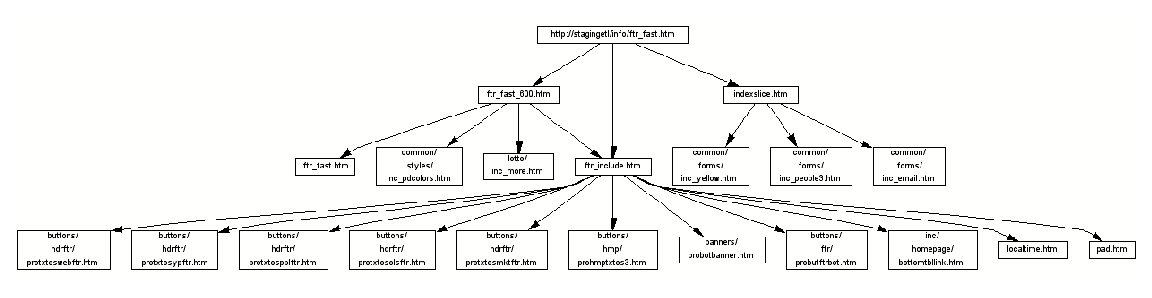
\includegraphics[width=1.06\linewidth]{ftr_fast-call-graph.eps}
\caption{This call-graph of templates possibly used in generating an HTML
page footer was extracted using server-side XPath expressions and a
simple Perl script. \label{fig-call-graph}}
\end{centering}
\end{figure*}


%%% 
\section{Implementation \& experience}
\label{sec-implementation}

A byte-code compiler and runtime for the Extensible Templating Language is
an integral part of InfoSpace's ETL Server 2.0.  ETLS is architected as an
ISAPI extension to Microsoft's IIS and could be easily ported to any
web server that exposes a similar Extension Control Block interface.
IIS is used to manage the raw socket connections and many HTTP
protocol details, but ETLS generates the response for all incoming
requests (including static files which are still subject to template
selection rules~\ssecref{selection}).

In addition to supporting the ETL language, our secondary design goals
in building ETLS were: 1) to be an appliance network box, so that all
interactions with the server could occur via simple network protocols
such as HTTP and SMB fileshares; 2) support easy management via HTTP
and platform specific management interfaces such as the Microsoft
Management Console (MMC) and the Service Control Manager; 3) to
provide support for secure debugging and run-time reflection on 
template execution.

\begin{figure}[tb]
\begin{centering}
\hspace*{-0.05\linewidth}\includegraphics[width=1.1\linewidth]{etls-admin-screenshot.eps}
\caption{The ETL Server has a web-based administration interface to
support configuration and management.
\label{fig-etls-admin}}
\end{centering}
\end{figure}

To meet the needs for administrative management of the server, we
implemented special primitives in the \smtexttt{admin} namespace that
expose reflection and configuration capabilities.  For example,
\smtexttt{admin:show-urlcache} generates an XML dump of the state of
the cached URL to template mapping and \smtexttt{admin:reset-urlcache}
resets that cache.  These special primitives are only available when
the request being served is properly authenticated and authorized
(e.g., by originating on distinguished port that is blocked at the
networking level from access by the Internet at large).  To facilitate
easy management of the server, we implemented a web application (in
ETL, of course) that organizes and exposes these underlying primitives
and integrates the documentation for the server (see
\figref{etls-admin}).  All server parameters are settable via
\smtexttt{admin:*} primitives, and the server is bootstrapped and
configured by executing a distinguished \smtexttt{etl-server-conf.etl}
template prior to handling HTTP requests.

To facilitate debugging, ETLS supports numerous special URL
parameters, each prefixed with \smtexttt{etl-}, that enable special
processing of the request.  As with the special primitives, these
extra behaviours function only when the request is authenticated and
authorized. For example, \smtexttt{?etl-show-resolution} suppresses
the normal response document and instead generates an XML document
that describes the dynamic call graph used in servicing the request.
Another parameter, \smtexttt{?etl-decompile} can be added to a URL to
request that the server dump the internal byte-compiled representation
as the response (see \figref{etl-decompile}).  Other parameters, such
as \smtexttt{?etl-no-random} and
\smtexttt{?etl-dummy-ads}, simplify testing by making eliminating some
major points of non-determinism in template execution.  These
capabilities enormously simplify confirming that web applications
behave the same as templates or the server itself are changed.

\begin{figure}[htbp]
\begin{smallverbatim}
Template `books.html.etl' has 0 errors.
0 template('books.html.etl') {
1  set_simple(#xml/books := '...')
2  #nocmd('<html>','</html>') {
3   #nocmd('<table>','</table>') {
4    for-each(#xml/books/book) {
5     #nocmd('<tr>','</tr>') {
6      #nocmd('<td>','</td>') {
7       get(@author)
       } // #nocmd('<td>','</td>')
8      #nocmd('<td>','</td>') {
9       get(@title)
       } // #nocmd('<td>','</td>')
      } // #nocmd('<tr>','</tr>')
     } // for-each(#xml/books 'book')
    } // #nocmd('<table>','</table>')
   } // #nocmd('<html>','</html>')
  } // template('books.html.etl')
\end{smallverbatim}
\caption{To support debugging, the ETL server permits decompilation of
the internal representation of the ETL template from
\figref{etl-books}.  The nesting of elements 
is preserved, but the byte-codes have been linearized for performance.
\label{fig-etl-decompile}}
\end{figure}

Although the special \smtexttt{etl-*} parameters are very valuable,
often single-stepping through code or using breakpoints still is the
best way to track down specific problems.  To that end, we built an
ActiveX-based debugger (\figref{debugger-screenshot}) that embeds
itself in Internet Explorer and communicates with the ETL server via a
separate persistent TCP connection.  It supports single stepping (both
forwards and backwards) as well as the setting of breakpoints and the
inspection of variables and request parameters.  The debugger also
provides a convenient display mechanism for trace messages (output
using \smtexttt{bl:trace} and other warning messages that would
normally be sent to the standard-error output.

\begin{figure}[tb]
\begin{centering}
\hspace*{-0.03\linewidth}\includegraphics[width=1.1\linewidth]{debugger-screenshot.eps}
\caption{The ETL debugger is an important part of making the
ETL development experience comparable to templates built on top of a
general-purpose programming language.
\label{fig-debugger-screenshot}}
\end{centering}
\end{figure}

InfoSpace's production web tree contains over sixty thousand ETL
templates and the clusters of ETL Servers serve over forty million
requests per day.  The templates were generated by a complex
multi-step automatic migration process from a lower level proprietary
templating language that pre-dates ETL.  The automatic migration was
made possible by the fact that the preceding language, too, was very
restrictive on the language level constructs it afforded.  However,
that language, like ASP and JSP, was text-based, not markup-based, and
used a proprietary and obscure syntax that made writing tools and
analyzing the source code especially troublesome.  

As part of migrating from our legacy language to ETL, we wrote a
lint-style checker to uncover ambiguities in the original source
templates.  That script uncovered about forty-five thousand total
major warnings spanning about fourteen thosand templates that required
a human to resolve an ambiguity or an error. Fortunately, most of the
corrections were straightforward and the entire process only took a
couple of months of background processing by our web development
teams.

Thus far, only a couple hundred templates have been authored directly
in ETL outside of the server development team.  Most notably the
administration interface was written using the tools described above,
and the feedback from those web developers has been extraordinarily
positive.

%%% 
\section{Related work}
\label{sec-related-work}

\gjb{write these up nicely}

JavaML -- key observation is that folks are already writing XML when
doing markup templating, so it is a natural place to apply the
benefits of an XML-based program representation.  Cite Zou \&
Kontogiannis; Power \& Malloy; Maletic, Collard, \& Marcus; Schonger,
Pulvermiller \& Sarstedt; 

XSLT -- declarative and that confuses folks.  Plus too limited in
terms of ability to interact with external components -- you end up
having to use a mix of XSLT and a scripting language with all the
problems that entails.  Also, no streaming mechanism -- a DOM is built-up
internally then serialized.~\cite{XSLT}

LAML -- the dual of ETL -- took markup and embedded it in Scheme,
whereas ETL takes only the most critical programming constructs and
embeds them in XML.  Mention S-exp and XML similarity.~\cite{Laml,Laml-WWW2002}

Modeling HTML in Haskell \& Typed representation for HTML \& XML in
Haskell, WASH. Web Scripting in
Curry.~\cite{Thiemann2002,Meijer2000,Meijer2001,Hanus2001}

BigWig -- similar goals, but take a general purpose programming
language and extend it with a first class markup fragment type with
gaps that can be plugged.  They do lattice-theoretic iterative
data-flow analyses, ETL focuses on practical aspects of limiting
common mistakes:  it'd be interesting to apply the data flow analyses
to ETL to make it provably generate correct markup, but that wasn't an
a priori goal.~\cite{BigWig,Brabrand2001,Brabrand2002}

XExpr~\cite{XExpr}


%%% 
\section{Conclusions \& future work}
\label{sec-conclusion}

* Restate contribution, stress in actual use


** XML infoset and non-infoset artifacts
*** a bit problematic for source->source and for representing literal markup \cite{VanDeVanter2001}
** alternate syntax (a la stylescript) for other purposes
*** importantly, has an implied XML data model (e.g., can be algorithmically turned into the other syntax)
** math and conditionals
** generalized content-slot
** improvements to XSD to enable better validation
*** e.g., either/or attributes for slots
*** custom tag element definitions
** levels of strictness
** data flow analyses to infer needs for xmlencoding of variable values
** taint tracking of input variables
** better warning/error reporting in terms of the pre-macro-transformed source template

** Considering domain specific languages for bl:calc/@expr and bl:if/@test

\section{Acknowledgments}
\label{sec-ack}
This research is supported by InfoSpace and its advanced server
development group.  I thank Russ Arun and Steve Newman for their early
recognition of the value of this approach and their support.  ETL
itself was designed in collaboration with Abhishek Parmar and is
influenced by the legacy language of its predecessor web server which
was implemented by Jean-Remy Facq.  The ETL Server was built by the
author along with Abhishek Parmar, Venkatesh Juryala, Sridhar Koneru,
Mark Sandori, Michael Harrison, Kris Bradley, Angela Plyler, Sunil
Thomas, and Howard Zhao.  Testing of ETLS was ably performed by Zine
Rif, Sriram Krishnan, Michael Schaffer, Shavkat Azimov, Jeff Wells,
Ilian Georgeiw, and Russell Ashmun, and credit goes to Antonio
Casacuberta for continued support of the server group.  I also thank
Jeff Torgerson, Matthew Benedict, Vasanth Cattamanchi and all of the
InfoSpace web developers for their input and contributions to
the system. ETLS is a trademark of InfoSpace, Inc.


\bibliographystyle{abbrv}
\bibliography{etl-www2003}  % sigproc.bib is the name of the Bibliography in this case

%
%\balancecolumns
%\appendix
%Appendix A
%\section{}
%\balancecolumns % GM July 2000

\end{document}
